\section{Funcionalidades do sistema}

No que diz respeito às funcionalidades do sistema é necessário ter em conta a definição dos seus 
utilizadores e quais as objetivos que a aplicação se propõe a resolver.
Nesse sentido foram definidos três tipos de utilizadores cada um com um conjunto concreto de 
funcionalidades que lhes são fornecidas.
De forma a conseguir fazer este tipo de especificação foram idealizados os seguinte tipos de utilizadores
que interagirão com o sistema, sendo eles: utilizador não registado e utilizador registado na forma de 
docente e aluno.

\begin{figure}[H] 
   \centering
   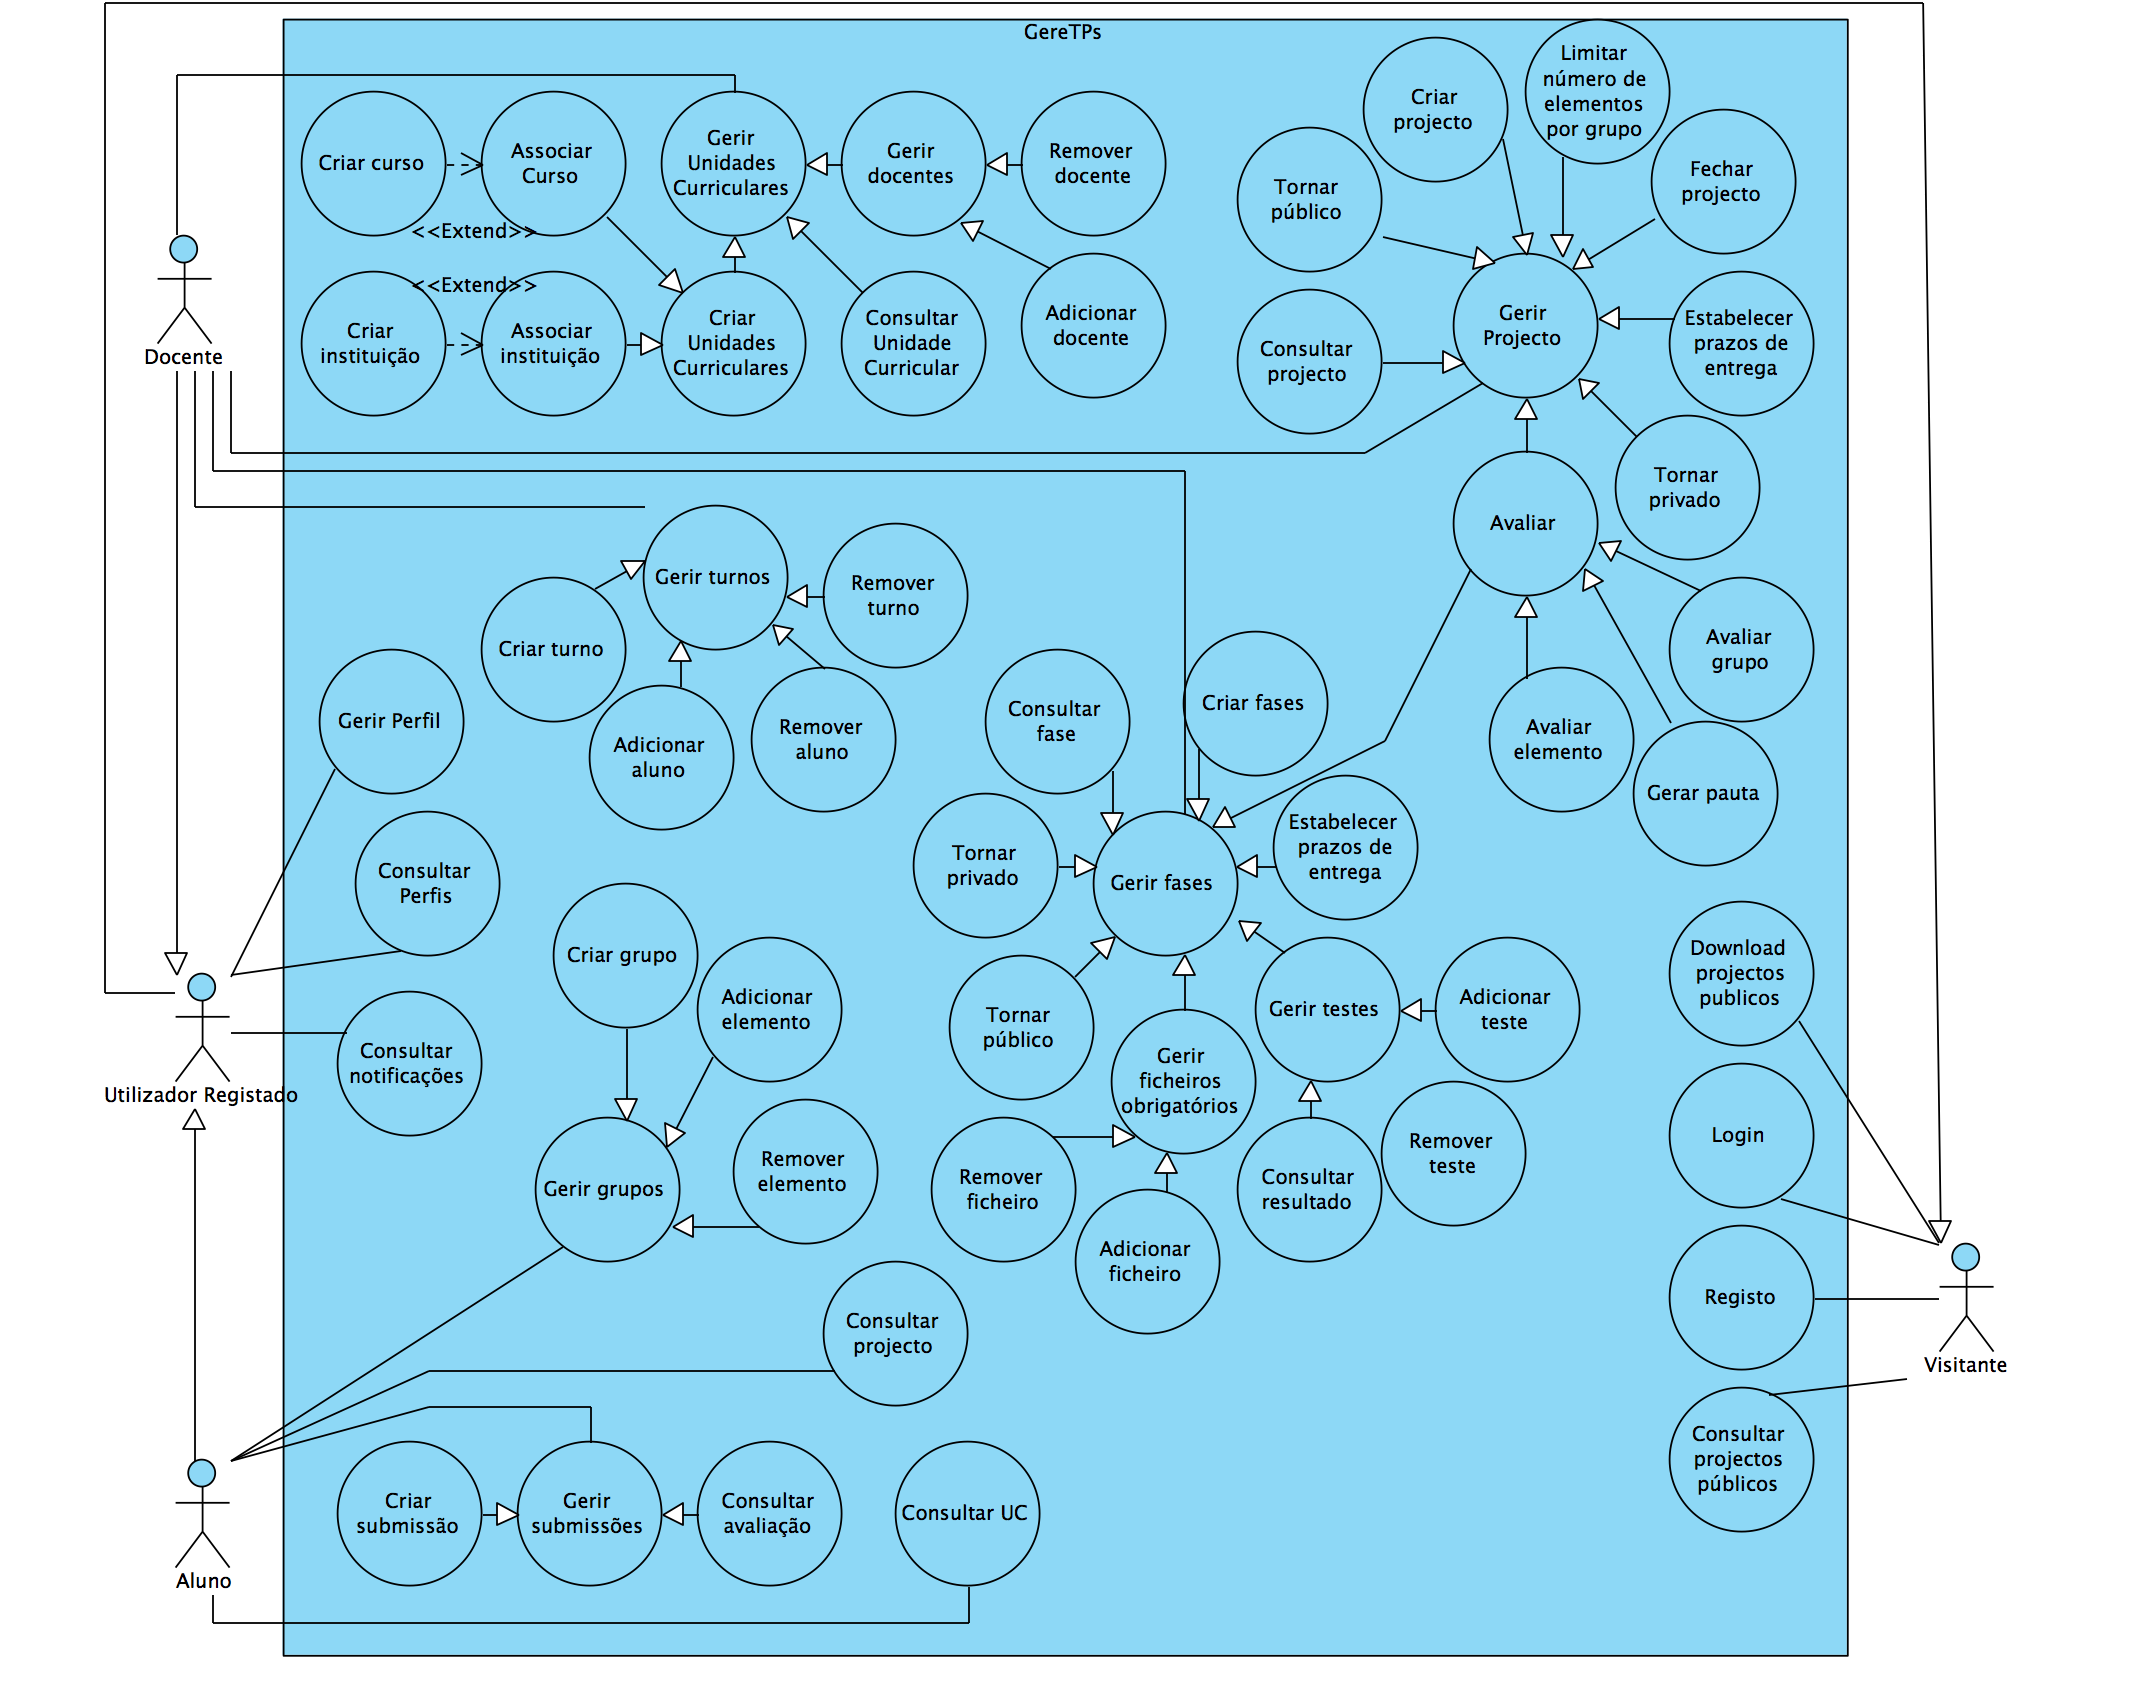
\includegraphics[width=1\textwidth]{images/funcionalidades/usecases.png}
    \caption{Diagrama com casos de uso dos utilizadores do sistema}
    \label{fig: usecases}
 \end{figure}

\subsection{Utilizadores não registados}

Como é possível ver no diagrama de Casos de uso representado na Figura \ref{fig: usecases}, no caso 
dos Utilizadores não registados, representados no diagrama pelo ator Visitante, são disponibilizadas
funcionalidades de registo, entrada no sistema, consulta e \textit{download} de projetos públicos.

Assim sendo é permitido a este tipo de utilizadores registarem-se na aplicação, providenciando informações
pessoais e criando então uma conta persistente com os seus dados, definindo-se a si próprio como
docente ou aluno. Após o registo é-lhes permitida a entrada no sistema com as credenciais de acesso
definidas aquando do registo prévio. Como utilizadores não registados podem também consultar e procurar
todos os projetos disponibilizados por outros utilizadores na aplicação, assim como também lhes é fornecida
a opção de descarregarem os mesmos projetos para o dispositivo de onde acessam.

\subsection{Docentes}

O seguinte tipo de utilizadores descrevem-se como utilizadores registados, sendo-lhes 
disponibilizadas funcionalidades específicas dentro do ambiente da aplicação. Nesse sentido, para 
além de serem uma extensão de Utilizadores não registados após o registo, são-lhes conferidas um
grupo de funcionalidades adicionais que descrevem o comportamento deste tipo de utilizador.

A um docente são disponibilizados quatro grupos de funcionalidades, como é possível observar na Figura
\ref{fig: usecases}. Esses grupos de funcionalidades são a gestão de unidades curriculares, turnos, 
projetos e fases.

No que diz respeito à gestão de unidades curriculares é tornado possível a este tipo 
de utilizador vários tipos de ações sobre as mesmas, nomeadamente, a consulta, a criação e 
remoção, a gestão de docentes, atualização das informações associadas, entre 
outras.

Para além disso, dentro de uma unidade curricular também é possível proceder-se 
à gestão de turnos. Nesse aspeto, é providenciado ao docentes tarefas como consulta, 
criação e remoção de turnos bem como a adição e remoção de alunos desses mesmo 
turnos.

Relativamente à gestão dos projetos de uma unidade curricular são fornecidas 
aos docentes as ferramentas para a consulta, criação e remoção, publicação, 
estabelecimentos de prazos assim como limitações ao número de elementos de um 
grupo, avaliação de um elemento ou grupo e por fim para geração de pautas, de 
todos os projetos associados a uma unidade curricular onde o docente seja 
responsável.

Por fim, a gestão de fases de um projeto é definida por funcionalidades como a 
sua criação e remoção, consulta, tipo de visibilidade, definição de 
obrigatoriedade de ficheiros, definição de testes sobre entregas e estabelecimento de prazos limite 
para submissões.

\subsection{Alunos}

Tal como o tipo de utilizador Docente, o tipo de utilizador Aluno é uma extensão 
de um utilizador não registado após o registo. Este tipo de utilizador é 
definido pelas funcionalidades que lhe são disponibilizadas pelo sistema. Dentro 
destas funcionalidades podemos destacar um conjunto delas, nomeadamente a 
consulta de projetos e unidades curriculares, a gestão de grupos e de submissões de projetos.

No que diz respeito à gestão de grupos é possível um aluno criar um grupo dentro 
de um projeto e adicionar e remover outros alunos como elementos do grupo.

Para além disso também são disponibilizadas ferramentas na aplicação que permite 
aos alunos fazerem submissões ou entregas de projetos dentro de uma unidade 
curricular de onde façam parte de um dos turnos. Para além disso também lhes é 
possível consultar as avaliações dadas pelos docentes às suas submissões assim 
como consultar a unidade curricular e as pautas da mesma.

\newpage
